
%% bare_conf.tex
%% V1.4b
%% 2015/08/26
%% by Michael Shell
%% See:
%% http://www.michaelshell.org/
%% for current contact information.
%%
%% This is a skeleton file demonstrating the use of IEEEtran.cls
%% (requires IEEEtran.cls version 1.8b or later) with an IEEE
%% conference paper.
%%
%% Support sites:
%% http://www.michaelshell.org/tex/ieeetran/
%% http://www.ctan.org/pkg/ieeetran
%% and
%% http://www.ieee.org/

%%*************************************************************************
%% Legal Notice:
%% This code is offered as-is without any warranty either expressed or
%% implied; without even the implied warranty of MERCHANTABILITY or
%% FITNESS FOR A PARTICULAR PURPOSE! 
%% User assumes all risk.
%% In no event shall the IEEE or any contributor to this code be liable for
%% any damages or losses, including, but not limited to, incidental,
%% consequential, or any other damages, resulting from the use or misuse
%% of any information contained here.
%%
%% All comments are the opinions of their respective authors and are not
%% necessarily endorsed by the IEEE.
%%
%% This work is distributed under the LaTeX Project Public License (LPPL)
%% ( http://www.latex-project.org/ ) version 1.3, and may be freely used,
%% distributed and modified. A copy of the LPPL, version 1.3, is included
%% in the base LaTeX documentation of all distributions of LaTeX released
%% 2003/12/01 or later.
%% Retain all contribution notices and credits.
%% ** Modified files should be clearly indicated as such, including  **
%% ** renaming them and changing author support contact information. **
%%*************************************************************************


% *** Authors should verify (and, if needed, correct) their LaTeX system  ***
% *** with the testflow diagnostic prior to trusting their LaTeX platform ***
% *** with production work. The IEEE's font choices and paper sizes can   ***
% *** trigger bugs that do not appear when using other class files.       ***                          ***
% The testflow support page is at:
% http://www.michaelshell.org/tex/testflow/



\documentclass[conference]{IEEEtran}
% Some Computer Society conferences also require the compsoc mode option,
% but others use the standard conference format.
%
% If IEEEtran.cls has not been installed into the LaTeX system files,
% manually specify the path to it like:
% \documentclass[conference]{../sty/IEEEtran}





% Some very useful LaTeX packages include:
% (uncomment the ones you want to load)


% *** MISC UTILITY PACKAGES ***
%
%\usepackage{ifpdf}
% Heiko Oberdiek's ifpdf.sty is very useful if you need conditional
% compilation based on whether the output is pdf or dvi.
% usage:
% \ifpdf
%   % pdf code
% \else
%   % dvi code
% \fi
% The latest version of ifpdf.sty can be obtained from:
% http://www.ctan.org/pkg/ifpdf
% Also, note that IEEEtran.cls V1.7 and later provides a builtin
% \ifCLASSINFOpdf conditional that works the same way.
% When switching from latex to pdflatex and vice-versa, the compiler may
% have to be run twice to clear warning/error messages.






% *** CITATION PACKAGES ***
%\usepackage{cite}

% cite.sty was written by Donald Arseneau
% V1.6 and later of IEEEtran pre-defines the format of the cite.sty package
% \cite{} output to follow that of the IEEE. Loading the cite package will
% result in citation numbers being automatically sorted and properly
% "compressed/ranged". e.g., [1], [9], [2], [7], [5], [6] without using
% cite.sty will become [1], [2], [5]--[7], [9] using cite.sty. cite.sty's
% \cite will automatically add leading space, if needed. Use cite.sty's
% noadjust option (cite.sty V3.8 and later) if you want to turn this off
% such as if a citation ever needs to be enclosed in parenthesis.
% cite.sty is already installed on most LaTeX systems. Be sure and use
% version 5.0 (2009-03-20) and later if using hyperref.sty.
% The latest version can be obtained at:
% http://www.ctan.org/pkg/cite
% The documentation is contained in the cite.sty file itself.






% *** GRAPHICS RELATED PACKAGES ***
%
\ifCLASSINFOpdf
  \usepackage[pdftex]{graphicx}
  % declare the path(s) where your graphic files are
  \graphicspath{{../images/}}
  % and their extensions so you won't have to specify these with
  % every instance of \includegraphics
  \DeclareGraphicsExtensions{.jpg,.jpeg,.png}
\else
  % or other class option (dvipsone, dvipdf, if not using dvips). graphicx
  % will default to the driver specified in the system graphics.cfg if no
  % driver is specified.
  % \usepackage[dvips]{graphicx}
  % declare the path(s) where your graphic files are
  % \graphicspath{{../eps/}}
  % and their extensions so you won't have to specify these with
  % every instance of \includegraphics
  % \DeclareGraphicsExtensions{.eps}
\fi
% graphicx was written by David Carlisle and Sebastian Rahtz. It is
% required if you want graphics, photos, etc. graphicx.sty is already
% installed on most LaTeX systems. The latest version and documentation
% can be obtained at: 
% http://www.ctan.org/pkg/graphicx
% Another good source of documentation is "Using Imported Graphics in
% LaTeX2e" by Keith Reckdahl which can be found at:
% http://www.ctan.org/pkg/epslatex
%
% latex, and pdflatex in dvi mode, support graphics in encapsulated
% postscript (.eps) format. pdflatex in pdf mode supports graphics
% in .pdf, .jpeg, .png and .mps (metapost) formats. Users should ensure
% that all non-photo figures use a vector format (.eps, .pdf, .mps) and
% not a bitmapped formats (.jpeg, .png). The IEEE frowns on bitmapped formats
% which can result in "jaggedy"/blurry rendering of lines and letters as
% well as large increases in file sizes.
%
% You can find documentation about the pdfTeX application at:
% http://www.tug.org/applications/pdftex





% *** MATH PACKAGES ***
%
%\usepackage{amsmath}
% A popular package from the American Mathematical Society that provides
% many useful and powerful commands for dealing with mathematics.
%
% Note that the amsmath package sets \interdisplaylinepenalty to 10000
% thus preventing page breaks from occurring within multiline equations. Use:
%\interdisplaylinepenalty=2500
% after loading amsmath to restore such page breaks as IEEEtran.cls normally
% does. amsmath.sty is already installed on most LaTeX systems. The latest
% version and documentation can be obtained at:
% http://www.ctan.org/pkg/amsmath





% *** SPECIALIZED LIST PACKAGES ***
%\usepackage{algorithmic}
% algorithmic.sty was written by Peter Williams and Rogerio Brito.
% This package provides an algorithmic environment fo describing algorithms.
% You can use the algorithmic environment in-text or within a figure
% environment to provide for a floating algorithm. Do NOT use the algorithm
% floating environment provided by algorithm.sty (by the same authors) or
% algorithm2e.sty (by Christophe Fiorio) as the IEEE does not use dedicated
% algorithm float types and packages that provide these will not provide
% correct IEEE style captions. The latest version and documentation of
% algorithmic.sty can be obtained at:
% http://www.ctan.org/pkg/algorithms
% Also of interest may be the (relatively newer and more customizable)
% algorithmicx.sty package by Szasz Janos:
% http://www.ctan.org/pkg/algorithmicx




% *** ALIGNMENT PACKAGES ***
%
\usepackage{array}
% Frank Mittelbach's and David Carlisle's array.sty patches and improves
% the standard LaTeX2e array and tabular environments to provide better
% appearance and additional user controls. As the default LaTeX2e table
% generation code is lacking to the point of almost being broken with
% respect to the quality of the end results, all users are strongly
% advised to use an enhanced (at the very least that provided by array.sty)
% set of table tools. array.sty is already installed on most systems. The
% latest version and documentation can be obtained at:
% http://www.ctan.org/pkg/array


% IEEEtran contains the IEEEeqnarray family of commands that can be used to
% generate multiline equations as well as matrices, tables, etc., of high
% quality.




% *** SUBFIGURE PACKAGES ***
%\ifCLASSOPTIONcompsoc
%  \usepackage[caption=false,font=normalsize,labelfont=sf,textfont=sf]{subfig}
%\else
%  \usepackage[caption=false,font=footnotesize]{subfig}
%\fi
% subfig.sty, written by Steven Douglas Cochran, is the modern replacement
% for subfigure.sty, the latter of which is no longer maintained and is
% incompatible with some LaTeX packages including fixltx2e. However,
% subfig.sty requires and automatically loads Axel Sommerfeldt's caption.sty
% which will override IEEEtran.cls' handling of captions and this will result
% in non-IEEE style figure/table captions. To prevent this problem, be sure
% and invoke subfig.sty's "caption=false" package option (available since
% subfig.sty version 1.3, 2005/06/28) as this is will preserve IEEEtran.cls
% handling of captions.
% Note that the Computer Society format requires a larger sans serif font
% than the serif footnote size font used in traditional IEEE formatting
% and thus the need to invoke different subfig.sty package options depending
% on whether compsoc mode has been enabled.
%
% The latest version and documentation of subfig.sty can be obtained at:
% http://www.ctan.org/pkg/subfig




% *** FLOAT PACKAGES ***
%
\usepackage{fixltx2e}
% fixltx2e, the successor to the earlier fix2col.sty, was written by
% Frank Mittelbach and David Carlisle. This package corrects a few problems
% in the LaTeX2e kernel, the most notable of which is that in current
% LaTeX2e releases, the ordering of single and double column floats is not
% guaranteed to be preserved. Thus, an unpatched LaTeX2e can allow a
% single column figure to be placed prior to an earlier double column
% figure.
% Be aware that LaTeX2e kernels dated 2015 and later have fixltx2e.sty's
% corrections already built into the system in which case a warning will
% be issued if an attempt is made to load fixltx2e.sty as it is no longer
% needed.
% The latest version and documentation can be found at:
% http://www.ctan.org/pkg/fixltx2e


%\usepackage{stfloats}
% stfloats.sty was written by Sigitas Tolusis. This package gives LaTeX2e
% the ability to do double column floats at the bottom of the page as well
% as the top. (e.g., "\begin{figure*}[!b]" is not normally possible in
% LaTeX2e). It also provides a command:
%\fnbelowfloat
% to enable the placement of footnotes below bottom floats (the standard
% LaTeX2e kernel puts them above bottom floats). This is an invasive package
% which rewrites many portions of the LaTeX2e float routines. It may not work
% with other packages that modify the LaTeX2e float routines. The latest
% version and documentation can be obtained at:
% http://www.ctan.org/pkg/stfloats
% Do not use the stfloats baselinefloat ability as the IEEE does not allow
% \baselineskip to stretch. Authors submitting work to the IEEE should note
% that the IEEE rarely uses double column equations and that authors should try
% to avoid such use. Do not be tempted to use the cuted.sty or midfloat.sty
% packages (also by Sigitas Tolusis) as the IEEE does not format its papers in
% such ways.
% Do not attempt to use stfloats with fixltx2e as they are incompatible.
% Instead, use Morten Hogholm'a dblfloatfix which combines the features
% of both fixltx2e and stfloats:
%
% \usepackage{dblfloatfix}
% The latest version can be found at:
% http://www.ctan.org/pkg/dblfloatfix




% *** PDF, URL AND HYPERLINK PACKAGES ***
%
\usepackage{url}
% url.sty was written by Donald Arseneau. It provides better support for
% handling and breaking URLs. url.sty is already installed on most LaTeX
% systems. The latest version and documentation can be obtained at:
% http://www.ctan.org/pkg/url
% Basically, \url{my_url_here}.




% *** Do not adjust lengths that control margins, column widths, etc. ***
% *** Do not use packages that alter fonts (such as pslatex).         ***
% There should be no need to do such things with IEEEtran.cls V1.6 and later.
% (Unless specifically asked to do so by the journal or conference you plan
% to submit to, of course. )


% correct bad hyphenation here
\hyphenation{op-tical net-works semi-conduc-tor}


\begin{document}
%
% paper title
% Titles are generally capitalized except for words such as a, an, and, as,
% at, but, by, for, in, nor, of, on, or, the, to and up, which are usually
% not capitalized unless they are the first or last word of the title.
% Linebreaks \\ can be used within to get better formatting as desired.
% Do not put math or special symbols in the title.
\title{An Efficient Query Platform for Streaming and Dynamic Natural Graphs}


% author names and affiliations
% use a multiple column layout for up to three different
% affiliations
\author{\IEEEauthorblockN{Milindu Sanoj Kumarage}
\IEEEauthorblockA{University of Colombo School of Computing\\
Colombo, Sri Lanka\\
Email: Milindu.S.Kumarage@ieee.org}
\and
\IEEEauthorblockN{Dr. D.N.Ranasinghe}
\IEEEauthorblockA{University of Colombo School of Computing\\
Colombo, Sri Lanka\\
Email: dnr@ucsc.cmb.ac.lk}
}

% conference papers do not typically use \thanks and this command
% is locked out in conference mode. If really needed, such as for
% the acknowledgment of grants, issue a \IEEEoverridecommandlockouts
% after \documentclass

% for over three affiliations, or if they all won't fit within the width
% of the page, use this alternative format:
% 
%\author{\IEEEauthorblockN{Michael Shell\IEEEauthorrefmark{1},
%Homer Simpson\IEEEauthorrefmark{2},
%James Kirk\IEEEauthorrefmark{3}, 
%Montgomery Scott\IEEEauthorrefmark{3} and
%Eldon Tyrell\IEEEauthorrefmark{4}}
%\IEEEauthorblockA{\IEEEauthorrefmark{1}School of Electrical and Computer Engineering\\
%Georgia Institute of Technology,
%Atlanta, Georgia 30332--0250\\ Email: see http://www.michaelshell.org/contact.html}
%\IEEEauthorblockA{\IEEEauthorrefmark{2}Twentieth Century Fox, Springfield, USA\\
%Email: homer@thesimpsons.com}
%\IEEEauthorblockA{\IEEEauthorrefmark{3}Starfleet Academy, San Francisco, California 96678-2391\\
%Telephone: (800) 555--1212, Fax: (888) 555--1212}
%\IEEEauthorblockA{\IEEEauthorrefmark{4}Tyrell Inc., 123 Replicant Street, Los Angeles, California 90210--4321}}




% use for special paper notices
%\IEEEspecialpapernotice{(Invited Paper)}




% make the title area
\maketitle

% As a general rule, do not put math, special symbols or citations
% in the abstract
\begin{abstract}
With the hype of Big Data, we see Big Graph is also becoming trendy where relationships in massive scale data are used to build massive scale graphs and then analysed for more insightful information. On the other hand, stream processing gaining lot of attention as they provides a way of extracting information in real-time. In most of the scenarios, even an approximated results are good enough if they can be generated in real-time.

This research evaluates the currently available graph analysing frameworks and identifies their strengths and weaknesses. Then proposes a query platform model for streaming graphs by researching and evaluating techniques and approaches which can be used for building such query platform. 

Identifying graph summarization as a good technique for such a query platform and discovering TCM sketching as a graph summarizasion model which fits the needs, a model was implemented using TCM sketching and evaluated with different metrics like Average Relative Error, Number of Effective Queries, Effectiveness of Effective Queries, Confusion Matrix of queries on streaming graphs. Same was evaluated with dynamically changing graphs and natural graphs which follows power-low degree distribution.

Then the research propose extensions to the TCM model for automatic sketch creation while the graph is building and evaluates the success when using different sketch creation policies. Then the contribution of different queries on the accuracy of the automatic sketch creation was evaluated.

The research shows the proposed model could work well with streaming graphs, even when the case of natural graphs, and produce 80\% to 90\% present effective queries which had $ \pm3$ deviation from exact correct results. We could show the effectiveness of the effective queries are also as expected.\\
\end{abstract}

% no keywords



% For peer review papers, you can put extra information on the cover
% page as needed:
% \ifCLASSOPTIONpeerreview
% \begin{center} \bfseries EDICS Category: 3-BBND \end{center}
% \fi
%
% For peerreview papers, this IEEEtran command inserts a page break and
% creates the second title. It will be ignored for other modes.
\IEEEpeerreviewmaketitle



\section{Introduction}
% no \IEEEPARstart
Massive scale datasets are getting common in day-to-day business with the expansion of the internet. More and more devices getting connected, more and more services coming online, more and more data generated and at the same time, the need to work on these data is getting more and more prominent.


However, modern day datasets no longer fit into one computing node as the amount of collected data are enormously huge.  We need some kind of a grid with thousands of computing nodes which can work on the dataset parallely, which might be distributed even across many geographical areas but connected through a network, communicating and coordinate their actions.


In the other hand, mapping these data into graphs and using graph algorithms to query useful information out of these graphs is also a growing need. Business intelligence systems, anomaly detections systems and many more real world use cases with huge financial values exists which needs insights that could be extracted from the relationships in the graphs, which is not easy to extract from traditional databases. We know the story of Google, how it became the search giant with their PageRank\cite{PageRank} algorithm which makes use of graph relations to rank the web pages of the World Wide Web and to produce the users the most related web pages to their queries. In the same way, Facebook uses their social graph with trillion edges\cite{Facebook} to uncover new insights about their users, products, and interactions.


Businesses are happy to have a system which can do real-time analysis \cite{Vitria}, even if they produce approximate results. This need produced systems like Apache Spark and Apache Flink which are streaming frameworks which can listen to the data streams and do the needed  analysis in real-time. 


We saw the need of a graph analytic framework which can work with graph streams where the users can plug their data streams, map them to graph streams, let the graph build over time, and then analyse the graph for different informations by submitting different queries time to time.

\subsection{Graph Analysis Frameworks}
We started analysing the currently available graph analysis frameworks to understand their internal workings, how they handle large scale graphs, queries, etc. These frameworks usually falls into two categories, as

\begin{enumerate}
\item OLTP (Online Transaction Processing)
\item OLAP (Online Analytical Processing)
\end{enumerate}

Online Transaction Processing frameworks are graph databases characterized by a large number of short online transactions (INSERT, UPDATE, DELETE). Online Analytical Processing aggregated are graph databases with historical data, stored in multidimensional schemas and characterized by relatively low volume of transactions. Research interest of this research is towards Online Analytical Processing rather Online Transaction Processing. Therefore, we evaluated currently available OLAP frameworks here.

Most of the well known solution in the literature and industry are only capable of analysing graphs that no new vertices or edges are added to the graph over the time\cite{Pregel} \cite{Graphlab}. These type of graphs are called bounded graphs while the graphs where new vertices and edges are inserted  over the time are called unbounded graphs or streaming graphs\cite{Fennel}\cite{S-PowerGraph}.


Several of these solutions allow changing the graph structure, that is, how edges are connected to the vertices. These dynamically changing graphs are called dynamic graphs and others are called static graphs, where the graph structure does not change\cite{X-stream}.


\section{Graph summarization}
Graph summarization is an interesting area of graphs where we create a summary of a huge graph. We can then do our computation on the summary instead of the original graph, but what we get is an approximate result. See figure \ref{fig:Graph summarization}. 

\begin{figure}[!b]
\centering
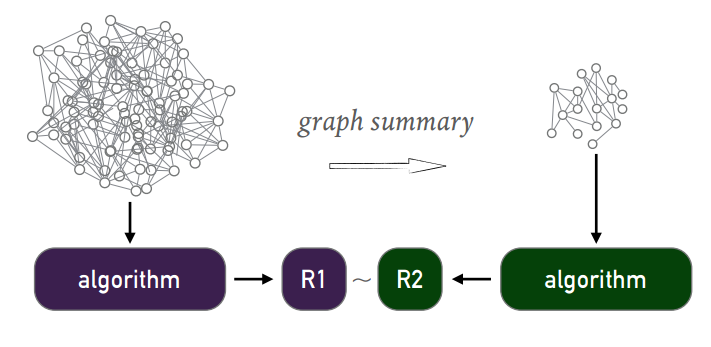
\includegraphics[width=\linewidth]{../images/image02}
\caption{Graph summarization and result approximation}
\label{fig:Graph summarization}
\end{figure}

Some highlighting properties of graph summarization are, 

\begin{enumerate}

\item $ | S_G | << | G |$ : the size of sketch $S_G$ is far less than the graph G, preferably in sublinear space.
\item The time to construct $S_G$ from G is in linear time.
\item The update cost of $S_G$ for each edge insertion/ deletion is in constant time.

\end{enumerate}


We evaluated several available graph summarization techniques in the literature and among them were different spanners\cite{sparse spanners}, sparsifiers\cite{Spectral sparsification}  and sketchers techniques. \cite{Graph stream algorithms survey} is a survey on these techniques.


Spanners and sparsifiers were left out as they were used mainly for distance estimation and cut estimation, and what needed was something which can represent the properties of original graph as a summary, not just distance or cuts.


Some example sketching techniques are frequency counts\cite{frequency counts}, Count-Min\cite{CountMin} and its variant gSketch\cite{gSketch}. But them both can support only a limited types of graph analytics, since they are not graphs. See figure \ref{fig:Count-Min}.

\begin{figure}[!b]
\centering
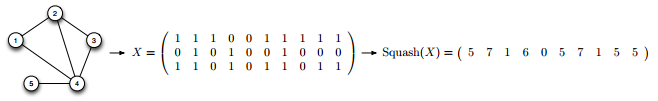
\includegraphics[width=\linewidth]{image15}
\caption{Count-Min's sketching technique visualized}
\label{fig:Count-Min}
\end{figure}


The problem with sketching is, like one pass algorithms, sketching are also query specific. However, TCM sketching promises the ability to use in general. 


\subsection{TCM Sketching}

TCM\cite{TCM} introduce a graphical sketch where a graph $S_G$(V, E), where V denotes the set of vertices and E its edges, is the summary of the graph G(V,E) and $|S_G| << |G|$. TCM promises a graph analytical method M which needs to run over a graph stream G, denoted as M(G), one can run it directly on its sketch $S_G$, M($S_G$), to get an approximate result, without modifying the method M.

\begin{figure}[!t]
\centering
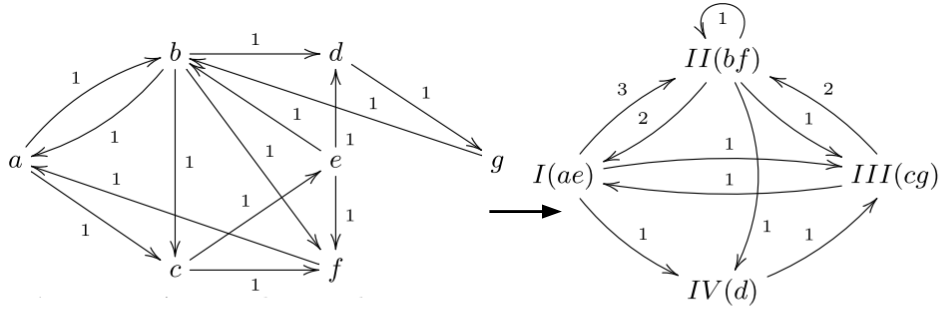
\includegraphics[width=\linewidth]{graph-sketching}
\caption{Example TCM sketch for a graph}
\end{figure}


In the TCM model, a sketch denotes an adjacency matrix of size m, which is called the sketch size. A set of such sketches are maintained, and when queried for information, the query is run on all the sketches simultaneously and the results from each sketch is merged to produced the final output. Merging the results of the sketches is done by using a aggregation function, which could be min(), max(), count() or any other. 


That is, for a given graph analytic method M to run on G, that is M(G), it is possible to run M on each n sketch separately, and then merge the result as follows, where $\tilde{M}(G)$ is the estimated result over G, and $\Gamma()$ is an aggregation function 


\begin{equation}
\tilde{M}(G) = \Gamma(M(S_1), ......., M(S_n))
\end{equation}

When an edge query is given, which can be denoted as $f_e(a,b)$ where a and b are node ids, the resulting approximated value, which is denoted as $\tilde{f}_e(a,b)$, could be calculated like as follows.

\begin{enumerate}
\item First  estimate edge weight $M_i[h(a)][h(b)] $ where $M_i[h(a)][h(b)]$ is the cell value relative to position h(a) and h(b) in adjacency matrix $M_i$ and h is the hash function.
\item Then uses a corresponding function $\Gamma()$ to merge the values from each matrix $M_i$.
\end{enumerate}
 
We can denote it as follows, 

\begin{equation}
\tilde{f_e}(a,b) = \Gamma(M_1[h(a)][h(b)], ......., M_n[h(a)][h(b)])
\end{equation}

You can see that estimating the aggregate weight of an edge query is in O(n) time, where n is a constant.


In the TCM paper they have shown how TCM enables to run all 4 types of graph analysis queries, which are nodes queries, edge queries, path queries and subgraph queries. 

We then implemented our graph query platform model using TCM sketching. More information could be found under next section.

% An example of a floating figure using the graphicx package.
% Note that \label must occur AFTER (or within) \caption.
% For figures, \caption should occur after the \includegraphics.
% Note that IEEEtran v1.7 and later has special internal code that
% is designed to preserve the operation of \label within \caption
% even when the captionsoff option is in effect. However, because
% of issues like this, it may be the safest practice to put all your
% \label just after \caption rather than within \caption{}.
%
% Reminder: the "draftcls" or "draftclsnofoot", not "draft", class
% option should be used if it is desired that the figures are to be
% displayed while in draft mode.
%
%\begin{figure}[!t]
%\centering
%\includegraphics[width=2.5in]{myfigure}
% where an .eps filename suffix will be assumed under latex, 
% and a .pdf suffix will be assumed for pdflatex; or what has been declared
% via \DeclareGraphicsExtensions.
%\caption{Simulation results for the network.}
%\label{fig_sim}
%\end{figure}

% Note that the IEEE typically puts floats only at the top, even when this
% results in a large percentage of a column being occupied by floats.


% An example of a double column floating figure using two subfigures.
% (The subfig.sty package must be loaded for this to work.)
% The subfigure \label commands are set within each subfloat command,
% and the \label for the overall figure must come after \caption.
% \hfil is used as a separator to get equal spacing.
% Watch out that the combined width of all the subfigures on a 
% line do not exceed the text width or a line break will occur.
%
%\begin{figure*}[!t]
%\centering
%\subfloat[Case I]{\includegraphics[width=2.5in]{box}%
%\label{fig_first_case}}
%\hfil
%\subfloat[Case II]{\includegraphics[width=2.5in]{box}%
%\label{fig_second_case}}
%\caption{Simulation results for the network.}
%\label{fig_sim}
%\end{figure*}
%
% Note that often IEEE papers with subfigures do not employ subfigure
% captions (using the optional argument to \subfloat[]), but instead will
% reference/describe all of them (a), (b), etc., within the main caption.
% Be aware that for subfig.sty to generate the (a), (b), etc., subfigure
% labels, the optional argument to \subfloat must be present. If a
% subcaption is not desired, just leave its contents blank,
% e.g., \subfloat[].


% An example of a floating table. Note that, for IEEE style tables, the
% \caption command should come BEFORE the table and, given that table
% captions serve much like titles, are usually capitalized except for words
% such as a, an, and, as, at, but, by, for, in, nor, of, on, or, the, to
% and up, which are usually not capitalized unless they are the first or
% last word of the caption. Table text will default to \footnotesize as
% the IEEE normally uses this smaller font for tables.
% The \label must come after \caption as always.
%
%\begin{table}[!t]
%% increase table row spacing, adjust to taste
%\renewcommand{\arraystretch}{1.3}
% if using array.sty, it might be a good idea to tweak the value of
% \extrarowheight as needed to properly center the text within the cells
%\caption{An Example of a Table}
%\label{table_example}
%\centering
%% Some packages, such as MDW tools, offer better commands for making tables
%% than the plain LaTeX2e tabular which is used here.
%\begin{tabular}{|c||c|}
%\hline
%One & Two\\
%\hline
%Three & Four\\
%\hline
%\end{tabular}
%\end{table}


% Note that the IEEE does not put floats in the very first column
% - or typically anywhere on the first page for that matter. Also,
% in-text middle ("here") positioning is typically not used, but it
% is allowed and encouraged for Computer Society conferences (but
% not Computer Society journals). Most IEEE journals/conferences use
% top floats exclusively. 
% Note that, LaTeX2e, unlike IEEE journals/conferences, places
% footnotes above bottom floats. This can be corrected via the
% \fnbelowfloat command of the stfloats package.

\section{Methodolgy}
\subsection{Evaluating TCM}

We wrote a web crawler which crawls the world wide web and create a graph stream about web pages and their links to other web pages. This graph stream used to continue with our testing on TCM. 


Visualizations of the building original graph and the sketches were created using a visualisation framework in order to get an idea. Several sketches with several sizes were created and visualized. Then started running different type of graph analysis queries on the sketches. 

\subsection{Dynamic querying}

However, our system had one limitation, that is, whenever wanted to run a new query the running process of building the graph had to be stooped and rerun changing the query. Then the graph starts building from the beginning which takes a lot of time, specially to become a  natural graph, showing power-low degree distribution. 


We followed two approaches here, one is we wrote our TCM implementation as a OSGi bundle, where we can keep the graph building and run any query on it dynamically, attaching to the graph. More about this could be found under next chapter. 


This way, we firstly deploy the TCM graph as a OSGi bundle to the OSGi platform and then we can submit a query as a OSGi bundle to the OSGi platform. OSGi bundles are compiled into JAR files, which we can dynamically load to the OSGi platform. 

\subsection{Simulation}

Other approach was to use Snapy.py which is a graph generation library by Stanford and generate a stream of graph and build the sketches.  With Snapy.py we can generate different types of graphs and with different degree distributions. This way, we could generate and analyse both random and natural graphs.

Number of sketches and the size of the sketches, that is the dimensions of the adjacency matrix of the sketch has a relation between how accurate the local and the final result for the analysis. Therefore, we tried generating different sketches, with different sizes and different number of sketches and continued to analyse the accuracy. 


We used a node query and plotted degree distribution of the vertices of the original graph and then used the same node query and plotted degree distribution of the vertices from the sketches. We then could compare the two plots to get an idea on the effects of sketches on the accuracy.  Then we performed a series of evaluations with TCM sketching. 

\subsection{Extending TCM}

One problem we understood with the TCM sketching was, we have to define the sketches beforehand. However, when working with the unbounded graphs, we don’t know how large the graph would grow. Because there is an relation between accuracy and number of sketches and sketch sizes, we saw the accuracy degrades when the graph is getting bigger. 


How TCM paper discuss to create a sketch is to take the full memory of the computation unit it is built on and create a sketch of that size and number of computation units available is how many sketches we create. However, when the graph is getting bigger, the accuracy keeps degrading. 


Creating a sketch of the size of the available memory is not a good solution in an era of cloud computation and distributed computing. We today is capable of vertically and horizontally scaling the resources available and pay as of the usage. We could start with 2GB of memory on one unit and scale up to 2TB of memory on 100s of units each.


As a graph analysis framework we have to handle this. This is a significant point where we have to come up with a novel idea to introduce extensions to the TCM model for automatic sketch creation. Thus we started investigation on this.

First we had to clarify what we consider as accuracy because definition of the accuracy is vague and changes with the type of the query. However, when looking at the fundamentals, we realized, the factor which relates to the accuracy of a TCM sketch is how many nodes of the original graph maps to a node of the sketch.


 For example, if the nodes of the original graph is as G[a,b,c,d,e,...] and nodes of sketch is as S[I, II, III, IV, ...,], when  we have only one node of original graph mapped to one node of sketch, as S[ I(a), II(b), III(c), IV(d),...], then the sketch is same as the original graph, whatever the query we run on sketch gives same results as the original graph. But when two nodes of the original graph shares one node of the sketch, as S[ I(a,e), II(b), III(c), IV(d),...], the accuracy might degrade. When more different nodes of the original graph maps to one node of the sketch is when the accuracy starts to fall. See figure \ref{fig:Example TCM sketch}.
 
\begin{figure}[!t]
\centering
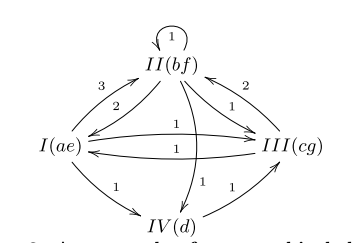
\includegraphics[width=0.8\linewidth]{example-tcm}
\caption{Example TCM sketch}
\label{fig:Example TCM sketch}
\end{figure} 


The main two problem was identifying when to create a new sketch and how to create a new sketch just by looking at the existing sketches. Since we hash the nodes to put into the sketches we have no way of reversing the hash and hashing again to the new sketch.


However, we realized we can solve our two main problems, when to create a new sketch and how to create a new sketch by looking at values returned from the sketches. For example, let's say we have 4 sketches with sizes as a, b, c, d where a \textless  b \textless c \textless d. When we query for an edge, each sketch returns the edge value as of that sketch and  we put these values to a list like this [ 7, 4, 3, 3 ] for instance, then what we do is, get the minimum value from the list, assuming it is the correct value and return as the result of that query.


At the beginning, for a given edge, the sketches might return something like [ 3, 2, 2, 2 ], but when the graph is growing, the smaller sketch will get more hash collisions, thus will return something like this, [ 7, 4, 3, 3  ]. We can understand looking at this, even though the correct value is 3 here, we have one sketch which gives the value as 7. When we see something like this, where some sketches are deviated from the correct value( minimum value ), then that is the correct time to create new sketches. 



We don't have to run edge queries for this explicitly, because when we insert an edge, we already query for the edge first to get the current value. This means we do not add overhead to the system and reading edge value is a constant time operation because what we do is read the adjacency matrix. When we think further, we thought we can delay creating a new sketch until it is only one sketch out of all sketches that return the correct value. We did several experiments on this, you can find the results under Results and Evaluation section.


Once we know when to create a new sketch, next problem we get is how to create a new sketch. Then we investigated how can we create new sketches using the knowledge we have at hand and we saw we can do it at the same time while checking whether we have to create a new sketch.


Let’s say while inserting an edge,  we decide to create a new sketch by looking at sketch values. We first create a new sketch with larger size and fill it with Nulls ( ∅ ). Let’s says  the sketch values were like this [ 7, 4, 3, 3 ]. From this sketch values we get the correct value as 3 and we can set the new sketch's value for that edge as 3, making the final sketch values list as  [ 7, 4, 3, 3, 3 ]. The next time we get an another query, we might get something like this for sketch values, [ 9, 3, 2, 2, ∅ ] because we have a new sketch and its matrix is filled with ∅s mostly. Now we omit the ∅ and get 2 as the correct value and then we set the new sketch’s adjacency matrix’s corresponding cell with that value. This way, we eventually fill the new sketches with very less overhead.  


We implemented this automatic sketch creating mechanism and tested for the accuracy with different measures. We firstly passed an array of sketch sizes in ascending order as parameters and let the sketches create automatically, but using the first two sketch sizes as the starting sketches. Then we identified how many sketches used by the system to store the given graph stream. Then we did the experiment giving the same graph stream but instead of creating the sketches dynamically, we created the the same number of sketches with the same sketch sizes at the beginning, like previous experiments.



Then we compared the outputs against the original graph and against each other. Then we compared the created sketches in both mechanisms and calculated how the sketches has deviated in the auto sketch creating technique  than the non auto sketch creating technique. You can find more details on this under the Results and Evaluation chapter. 



In this experiment the program waited until it is just one sketch that is giving the right value to create a new sketch as we described above. We could use several other techniques like this. We see these as automatic sketch creation policies. We tried several such policies and the evaluated the results. 



Some such policies we tried are, without waiting until it is just one sketch giving the correct results, we tried with waiting until it is only 2 sketch giving the correct results, only 3 sketches giving the correct results, half of the sketches giving the correct results, ¼ of the sketches giving the correct results, etc.  You can find more details on this under the Results and Evaluation chapter.


Then we tried tolerating errors upto a limit, that is, when there is only one sketch giving the correct result, say ‘v’, we checked how many sketches are having ‘v+1’ as the sketch value. If we have one or more sketches giving ‘v+1’, then we do not create a sketch. This is useful when we do not need exact values to be in sketches, but something very approximate. We call this the tolerance, where 1-tolerance means if the correct value is ‘v’ but when we have a ‘v+1’ in the sketch values we do not create a new sketch, and 2-tolerance means we do not create a sketch when we have a ‘v+1’ or ‘v+2’ in the sketch values. In our implementation we defined n-tolerance where the user can define the tolerance they need. 



We can have tolerance with different policies, like  only 2 sketches giving the correct results + 2-tolerance. Then the system check if at least 2 sketch values have either ‘v’ or ‘v+1’ or ‘v+2’ if the correct value is ‘v’. We did a series of tests with different combinations and evaluated the accuracy of the queries. You can find more details on this under the Results and Evaluation chapter.


Since we are building a framework, we should give the users to choose which policy suits for them. Therefore, in our implementation, we have a parent class as ‘SketchCreationPolicy’ and several sketch creation policies implemented as child classes of it. This way, the user can use whatever the sketch creation policy they like when setting up the graph or write their own sketch creation policy by extending the ‘SketchCreationPolicy’ class. More on this can be found under the Implementation chapter.



We have a problem when creating the initial sketch or sketches as we lacks knowledge on the graph stream's velocity, that is how many edges get inserted in a unit time. The solution we used is to listen to the stream for a time and count the edges and nodes we see within that time. We then multiply the number of nodes into a scaling factor and use that size as the initial sketch size. The time and the scaling factor is configurable in the system.



\newpage

\section{Evaluation}
In this section, evaluation of the proposed model, the results and the important parts of the implementation are discussed. Java was chosen as the implementation language as of the vast set of tools available and abundance community and references. The experiments was performed on a Intel i5 1.6Ghz machine with 8GB of RAM, running Ubuntu 14.4.

\subsection{Natural graphs from Webcrawler}
Following is a web graph generated by mapping the data stream of our web crawler as a graph stream and then built the graph. Each node indicates a webpage on the World Wide Web and each edge indicates a hyperlink between two such webpages. On figure \ref{fig:A large web graph generated by our web-crawler} you can see some nodes having many hyperlink while some have only few. 

\begin{figure}[!t]
\centering
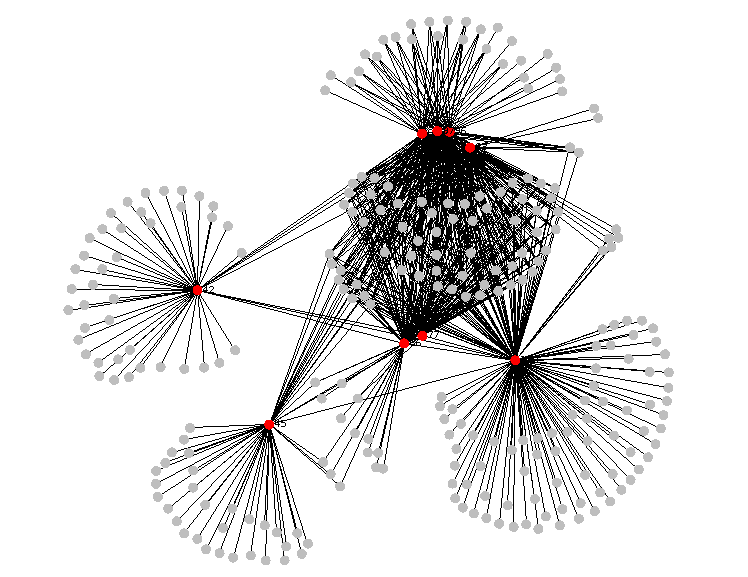
\includegraphics[width=\linewidth]{web-graph}
\caption{A large web graph generated by our web-crawler}
\label{fig:A large web graph generated by our web-crawler}
\end{figure}

It took us about half an hours to build this graph because crawling the web and fetching the hyperlinks from the webpage’s contents by parsing the HTML is a time consuming task. 


Following is same as above graph, but a zoomed out view and with many more nodes. The red dots you see are actually groups of nodes connected together. Edges has been removed for clarity but you can get an idea about the connectivity of nodes by the closeness of the nodes. You can see there are some nodes which has very high connectivity, thus forming big groups, like the one in the top left corner. 

\begin{figure}[!t]
\centering
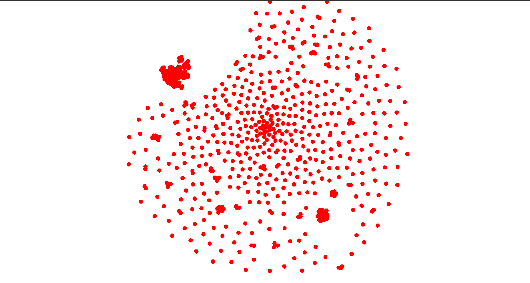
\includegraphics[width=\linewidth]{graph2}
\caption[Zoomed out view of a large web graph]{Zoomed out view of a large web graph generated by our web-crawler}
\end{figure}

\subsection{TCM Sketching}
While creating the above graph, three sketches were created, but with very small sketch sizes, only to get a visual representation of the sketches. First one is a sketch of size 12, see figure \ref{fig:A sketch of size 12}. The second one is a sketch of size 112, see figure \ref{fig:A sketch of size 112}.


\begin{figure}[!t]
\centering
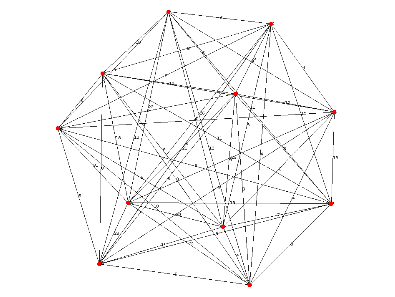
\includegraphics[width=0.6\linewidth]{s1}
\caption{A sketch of size 12}
\label{fig:A sketch of size 12}
\end{figure}


\begin{figure}[!t]
\centering
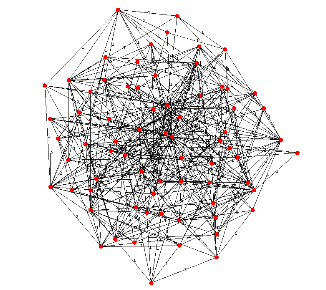
\includegraphics[width=0.6\linewidth]{s3}
\caption{A sketch of size 112}
\label{fig:A sketch of size 112}
\end{figure}

Next move was to use the sketches and query the graph. TCM paper has defined 4 types of queries and evaluated with several experiments. Node queries were chosen to start with as interesting queries like identifying top-k heavy hitters\cite{HeavyHitters}, conditional heavy hitters\cite{TCM}, etc are based on node queries, and then the edge queries are also evaluated.



We used small to medium scale graphs for initial testing, which ranges from 100 to 10,000 nodes and 1000 to 1,00,000 edges.  We did series of investigations using the graphs generated with Snapy.py \footnote{https://snap.stanford.edu/} using different configurations in generating graphs and sketches.


The most simplest node query is to ask the degree of a node giving a node id. What the experiment followed was, instead of asking random nodes, every node’s degree was asked by issuing series of node queries and using that information, calculated the number of nodes which has a certain degree. This way a degree distribution of the graph could be plotted. The same was queried from the original graph and was plotted the same.


Figure \ref{fig:Degree distribution from sketches of sizes 75, 80, 83, 89} is a degree distribution plot of a graph with 100 nodes and 1000 edges. The dotted line indicate the correct degree distribution which is calculated from the original graph, while the line indicates the degree distribution calculated by querying the TCM sketches. Here have used sketches of sizes 75, 80, 83, 89. You can see, there is a slight deviation between the two graphs but the original shape is preserved. 

\begin{figure}[!t]
\centering
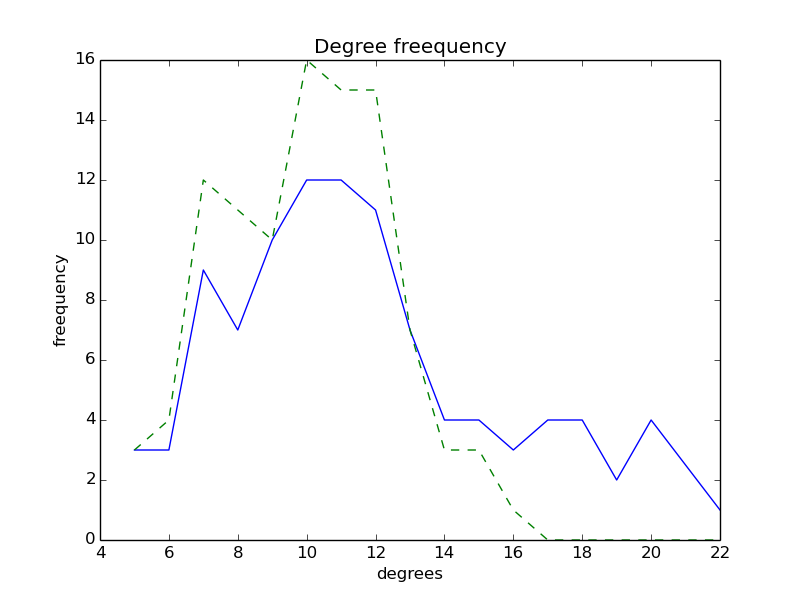
\includegraphics[width=\linewidth]{dd1}
\caption{Degree distribution from sketches of sizes 75, 80, 83, 89}
\label{fig:Degree distribution from sketches of sizes 75, 80, 83, 89}
\end{figure}

You can see a drop in the low degrees and a rise in the high degrees. This happens because of the small sketches having nodes which maps too many nodes of the original graph onto them, thus increasing the adjacency matrix’s corresponding cell value. When there are such nodes in the sketch, all the nodes of the original graph which maps to those nodes gives a higher values than they have. 


Next two graphs in figure \ref{fig:Degree distribution from sketches of sizes 89, 97} and figure \ref{fig:Degree distribution from sketches of sizes 85, 89, 97} are the same as figure \ref{fig:Degree distribution from sketches of sizes 75, 80, 83, 89} but with sketches  of sizes 89, 97 and 85, 89, 97 respectively. You can see how the degree distribution plot drawn from the TCM sketches has become more closer to the degree distribution plot drawn from the original graph. The bigger size of the sketches has contributed to more accurate results comparing previous plot and next two plots. By comparing the two graphs in figure \ref{fig:Degree distribution from sketches of sizes 89, 97} and figure \ref{fig:Degree distribution from sketches of sizes 85, 89, 97} you can see how more number of sketches has contributed to more accurate results.

\begin{figure}[!t]
\centering
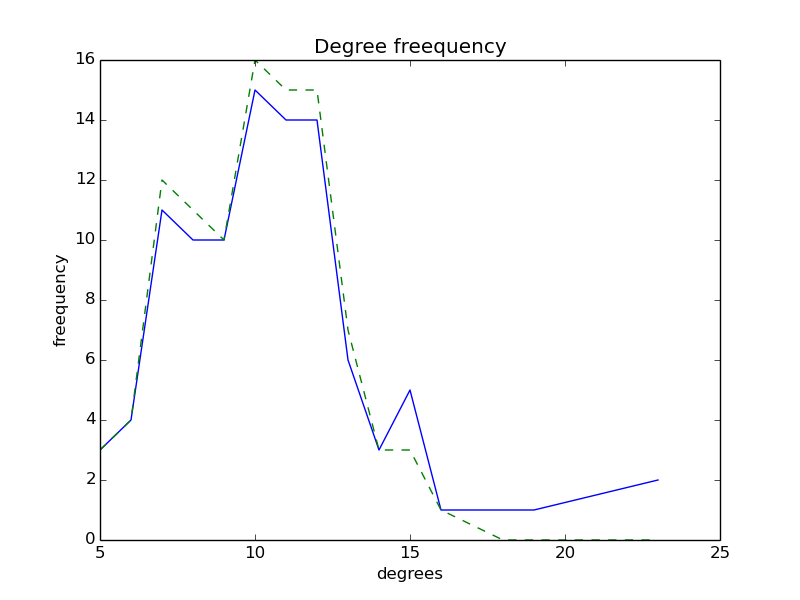
\includegraphics[width=0.8\linewidth]{dd2}
\caption{Degree distribution from sketches of sizes 89, 97}
\label{fig:Degree distribution from sketches of sizes 89, 97}
\end{figure}

\begin{figure}[!t]
\centering
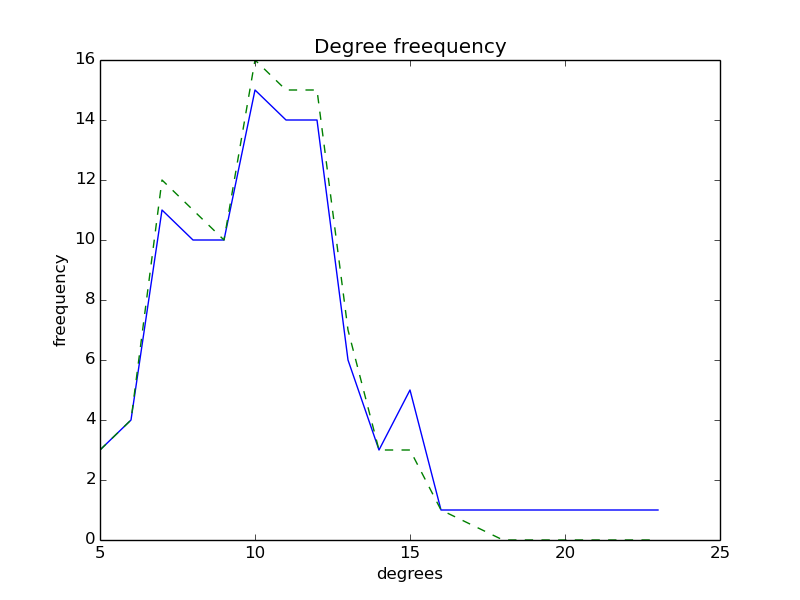
\includegraphics[width=0.8\linewidth]{dd3}
\caption{Degree distribution from sketches of sizes 85, 89, 97}
\label{fig:Degree distribution from sketches of sizes 85, 89, 97}
\end{figure}

\subsection{TCM Sketching for Natural graph}
Figure \ref{fig:Degree distribution of a streaming natural graph} is a plot of degree distribution of a natural graph, which was generated from our web crawler. The experiment time to time plotted the degree distribution of the graph by querying the sketches and from the original graph. The blue line indicate the correct degree distribution which is calculated from the original graph, while the red line indicates the degree distribution calculated by querying the TCM sketches. Here we have used sketches on sizes 10, 20, 70. You can see, there is a slight deviation between the two graphs but the original shape is preserved.

\begin{figure}[!t]
\centering
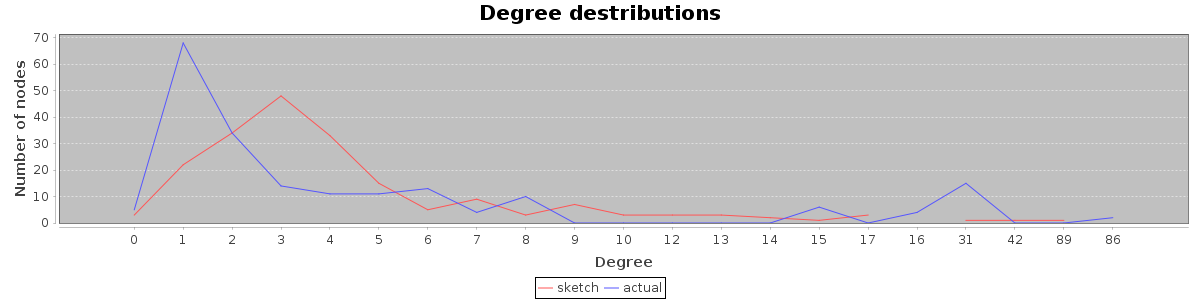
\includegraphics[width=\linewidth]{ddn}
\caption{Degree distribution of a streaming natural graph from sketches of sizes 10, 20, 70}
\label{fig:Degree distribution of a streaming natural graph}
\end{figure}

All the above experiments involved a series of node queries in each experiment and the results looked promising when visually compared. At this point, defining measures to evaluate the accuracy of the queries was needed. 

\subsection{Evaluation Metrics}
Number of queries running on the sketches giving the exact correct results as running on the original graph could be calculated easily, however, as the research is interested not only in exact correct results, but also in approximate results, this could not be used as a good measurement. Thus, better metrics were needed.


Average Relative Error and Number of Effective Queries was taken from gSketch\cite{gSketch} as TCM also has used Average Relative Error as a measurement. 

\subsubsection{Average Relative Error}
Average Relative Error is used for the set of queries that returns estimated frequencies, such as edge or node counts.


Relative error is defined as, 

\begin{equation}
er(Q) =  \frac{\tilde{f}'(Q) - f(Q)}{f(Q)} = \frac{\tilde{f}'(Q)}{f(Q)} -1 
\end{equation}


Given a set of m queries, $\{ Q_1 , ....., Q_m \}$, average relative error is defined by averaging the relative errors over all queries $Q_i$ for i ∈ [1,m] as,

\begin{equation}
e(Q) =  \frac{\sum_{i=1}^{k} er(Q_i)}{m}
\end{equation}

\subsubsection{Number of Effective Queries}
Average relative error could be biased measure if queries have significantly different frequencies. For instance, if an edge with low frequency happens to collide with another edge with very high frequency in the sketch, this will results in very large average relative errors. That is, a small number of such queries may dominate the overall average relative error in query estimation.


Here a query is said to be effective if the error, $\tilde{f}'(Q) - f(Q), < G_0$,  where $G_0$ is a predefined value. In our experiments, the number of queries which gives effective results having $G_0$ as 0, 1, 2, 3, 4 was calculated and then the percentage of such effective queries dividing by number of all queries, $|Q|$, performed was derived. 


\begin{equation}
g(Q) =  \frac{\left | \{\,q\, |   \left |\tilde{f}'(q) - f(q)\right | \leq G_0, \,q \, \epsilon  \,Q\} \, \right|}{|Q|}*100
\end{equation}

 
Then these metrics were used in the next set of experiments to measure the accuracy of the sketching. The same experiment as the previous ones was performed but with more nodes, edges and queries. This is because the metrics takes averages, and for averages to be unbiased, more trials were needed, which means more queries were needed.

\subsection{Evaluating with defined metrics}

This experiment was performed with 1000 nodes and 10,000 edges graph, and then running 1000 node queries on the graph. See figure \ref{fig:1000 nodes 10,000 edges with sketches of sizes 810, 820, 827, 830} for degree distribution plot.

\begin{figure}[!t]
\centering
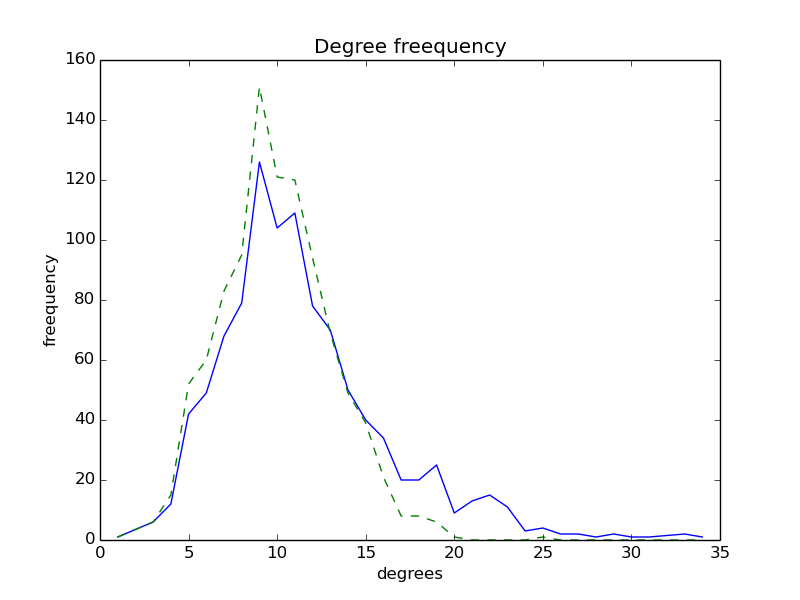
\includegraphics[width=0.7\linewidth]{n1000-e10000-sketches-810-820-823-827-830plot}
\caption[1000 nodes 10,000 edges with sketches of sizes 810, 820, 827, 830]{Degree distribution calculated on a graph with 1000 nodes 10,000 edges using set of sketches of sizes 810, 820, 827, 830}
\label{fig:1000 nodes 10,000 edges with sketches of sizes 810, 820, 827, 830}
\end{figure}

Then the metrics were calculated, which are Average Relative Error(ARE), Percentages of Effective Queries when $G_0$ is 0 (which is the number of queries giving the exact results), $G_0$ is 1, $G_0$ is 2 and $G_0$ is 3.

%\begin{table}[!t]
%% increase table row spacing, adjust to taste
%\renewcommand{\arraystretch}{1.3}
% if using array.sty, it might be a good idea to tweak the value of
% \extrarowheight as needed to properly center the text within the cells
%\caption{An Example of a Table}
%\label{table_example}
%\centering
%% Some packages, such as MDW tools, offer better commands for making tables
%% than the plain LaTeX2e tabular which is used here.
%\begin{tabular}{|c||c|}
%\hline
%One & Two\\
%\hline
%Three & Four\\
%\hline
%\end{tabular}
%\end{table}

\begin{table}[!b]
\caption{Accuracy metrics for sketching}
\label{table:accuracy-metrics-for-sketching}
\renewcommand{\arraystretch}{1.5}
\centering
\begin{tabular}{|c|c|c|c|c|}
\hline
 ARE   & $G_0$=0 & $G_0$=1 & $G_0$=2 & $G_0$=3 \\ \hline
0.163 &   82.6  &   82.8  &   82.8  &   83.5  \\ \hline
\end{tabular}
\end{table}


The experiment shows $82.6\%$ of the queries gave the exact same results and within $\pm3$ range approximation, there were $83.5\%$ queries giving correct results.


\subsection{Automatic sketch creation} 
In this experiment it was a graph with 1000 nodes and 10,000 edges was used with 'only two sketch gives correct value' policy with 0 tolerance and 2 initial sketches of sizes 810, 820. Automatic sketch creation mechanism had created altogether 5 sketches at the end with sizes 810, 820, 823, 827, 830.


Here the automatic sketch creation was firstly run and then the number of sketches created and their sizes used was identified. Then the same experiment was done with the used number of sketches and with their respective sizes. The accuracy metrics were as on table\ref{table:Accuracy metrics with automatic sketch creation}.


\begin{table}[!b]
\caption{Accuracy metrics with automatic sketch creation}
\label{table:Accuracy metrics with automatic sketch creation}
\centering
\begin{tabular}{|l|l|l|l|l|l|}
\hline
 ARE   & $G_0$=0 & $G_0$=1 & $G_0$=2 &  $G_0$=3 & $G_0$=4 \\ \hline
0.200 &   58.5  &  65.8   &   73.3  &   79.8   &   81.8 \\ \hline
\end{tabular}
\end{table}

Then the next experiment was done using the same number of sketches with same sizes, but without automatic creation, that is creating at the beginning. This way, we can benchmark the results of the automatic sketch creation with the results of the TCM with respect to accuracy measures. The accuracy metrics were as on table \ref{table:Accuracy metrics for sketching without auto sketch creation}.

\begin{table}[!b]
\caption{Accuracy metrics for sketching without auto sketch creation}
\label{table:Accuracy metrics for sketching without auto sketch creation}
\centering
\begin{tabular}{|l|l|l|l|l|l|}
\hline
 ARE   & $G_0$=0 & $G_0$=1 & $G_0$=2 & $G_0$=3 & $G_0$=4\\ \hline
0.172 &   80.9  &   81.1  &   81.9  &   82.3  & 83.3   \\ \hline
\end{tabular}
\end{table}

The resulted Average Relative Error from the experiment which used automatic sketch creation, which is 0.200 was reasonable when compared to Average Relative Error  of the experiment which did not used the automatic sketch creation. 


How the effective queries are distributed over the error space was plotted and it gave the idea that many queries were in a favourable error range and very few queries were much deviated.

\begin{figure}[!t]
\centering
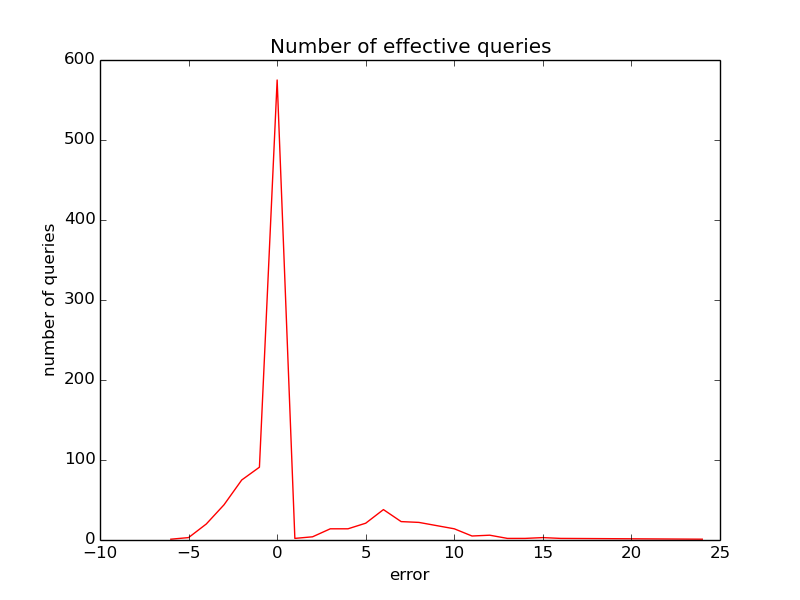
\includegraphics[width=\linewidth]{deviation-plot-AS-2init-2scale-0t-n1000-e10000-sketches-811-821-823-827-829-839plot}
\caption{ Effective queries against the error space }
\end{figure}

\subsection{Effectiveness of the effective queries }

Then the next question was, if these effective queries are really effective? Let's say a degree of a node is 12 and the query gives it as 10, that is within an error of 2, which is acceptable. Let's take this as case 1. But if a degree of a node is 3 and the query gives it as 1, which is still within an error of 2, then this might not be acceptable for some needs. Let's take this as case 2.


Then this was investigated using a plot which evaluates the frequency of approximated queries over the degrees. In Figure \ref{fig:Effective queries against degree}, frequency of effective queries when $G_0$ is 1 are marked with the green line, frequency of effective queries when $G_0$ is 2 are marked with the orange line, frequency of effective queries when $G_0$ is 1 are marked with the purple line. 


This shows us the queries which were considered as effective are how effective. The queries which were considered effective when $G_0 = 1$ is starting from degree 3, which means, it is only the case where 3 is approximated to 2, is reasonable. Even the frequency of such approximated queries are low for smaller degrees. Majority of the queries which are considered as effective by approximation are on higher degrees, which is the case like 12 getting as 10.

\begin{figure}[!t]
\centering
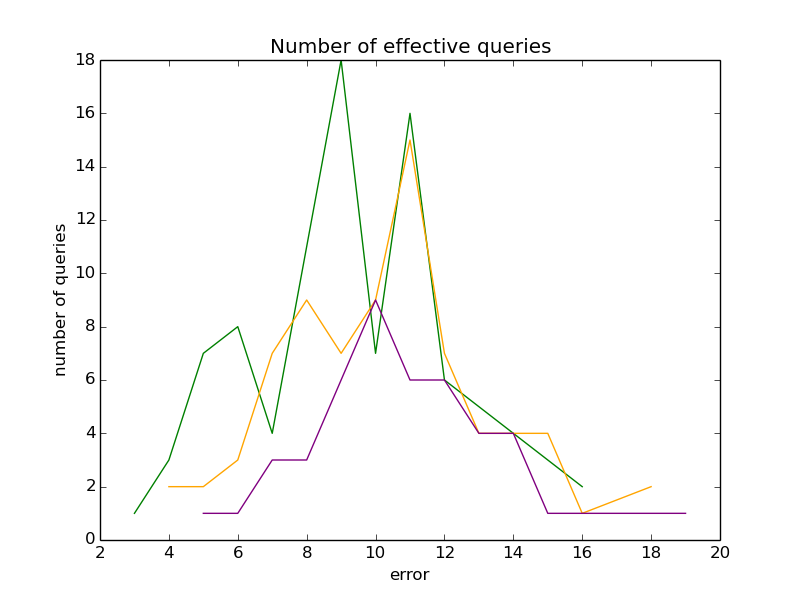
\includegraphics[width=\linewidth]{deviation-plot-error-AS-2init-2scale-0t-n1000-e10000-sketches-811-821-823-827-829plot}
\caption{ Effective queries against the degrees }
\label{fig:Effective queries against degree}
\end{figure}

\subsection{Evaluating different creating policies}

Different automatic sketch creation policies were then evaluated using a 1000 nodes and  10000 edges graph on sketches of sizes 810, 8210, 823, 827, 830 starting with 3 initial sketches. Following \ref{table:Accuracy metrics for sketching using 'only one sketch gives correct value'}, \ref{table:Accuracy metrics for sketching using 'only two sketch gives correct value'},  \ref{table:Accuracy metrics for sketching using 'only two sketch gives correct value' and 1 tolerance} tables holds some of the highlighting results. 


\begin{table}[!b]
\caption{Accuracy metrics for sketching using 'only one sketch gives correct value'}
\label{table:Accuracy metrics for sketching using 'only one sketch gives correct value'}
\centering
\begin{tabular}{|l|l|l|l|}
\hline
 ARE   & $G_0$=0 & $G_0$=1 & $G_0$=2 \\ \hline
0.299 &   40.1  &   48.6  &   57.6  \\ \hline
\end{tabular}
\end{table}


\begin{table}[!t]
\caption{Accuracy metrics for sketching using 'only two sketch gives correct value'}
\label{table:Accuracy metrics for sketching using 'only two sketch gives correct value'}
\centering
\begin{tabular}{|l|l|l|l|}
\hline
 ARE   & $G_0$=0 & $G_0$=1 & $G_0$=2 \\ \hline
0.200 &   57.5  &   66.8  &   77.7  \\ \hline
\end{tabular}
\end{table}


\begin{table}[!t]
\caption{Accuracy metrics for sketching using 'only two sketch gives correct value' and 1 tolerance}
\label{table:Accuracy metrics for sketching using 'only two sketch gives correct value' and 1 tolerance}
\centering
\begin{tabular}{|l|l|l|l|}
\hline
 ARE   & $G_0$=0 & $G_0$=1 & $G_0$=2 \\ \hline
0.406 &   62.7  &   62.7  & 63.1    \\ \hline
\end{tabular}
\end{table}

'Only two sketch gives correct value' with 0 or 1 tolerance gave better results in most of the experiments. On the 'only two sketch gives correct value' with 1 tolerance results above, the ARE is a bit higher than with 0 tolerance, the reason was there were several queries outside the  $G_0$=2 range which gave a bit higher deviated values.


\subsection{Experimenting with edge queries}

For the edge query experiment, the sketches were asked for the edge value giving two vertices. In the initial experiments, 10\% of the edges on the original graph were chosen randomly and then queried from the sketches. This way, when the graph has 1000 edges, 100 queries get performed in one experiment, and when graph has 10000 edges, 1000 queries get performed.

First experiment was done using 1000 nodes and 10000 edges and using sketches 145, 165, 170, 180. Number of Effective Queries were used as the accuracy measurements. Table \ref{table:Accuracy metrics for sketching with edge queries} holds the results of the initial experiment with edges.

\begin{table}[!b]
\caption{Accuracy metrics for sketching with edge queries}
\label{table:Accuracy metrics for sketching with edge queries}
\centering
\begin{tabular}{|l|l|l|}
\hline
$G_0$=0 & $G_0$=1 & $G_0$=2 \\ \hline
97.74  &   99.99  &   100.0\\ \hline
\end{tabular}
\end{table}

The results showed us the edge queries can produce quite accurate results using mush smaller sketches when compared to node queries. Then a series of experiment was performed with different edge sizes and the accuracy metrics were measured. Table \ref{table:Accuracy metrics for sketching with edge queries on series of experiments} holds some of the results.  

\begin{table}[!t]
\caption{Accuracy metrics for sketching with edge queries on series of experiments}
\label{table:Accuracy metrics for sketching with edge queries on series of experiments}
\centering
\begin{tabular}{|l|l|l|l|l|}
\hline
n    & e     & $G_0$=0 & $G_0$=1 & $G_0$=2 \\ \hline
1000 & 5000  & 99.44   & 100.00  & 100.00  \\ \hline
1000 & 10000 & 93.38   & 99.90   & 100.00  \\ \hline
1000 & 20000 & 66.25   & 95.57   & 99.77   \\ \hline
\end{tabular}
\end{table}

\subsection{Confusion matrix for edge queries}

The next question was if the sketches were asked for edges which does not exist in the actual graph, then can the sketches identify this. An experiment was performed using a graph of 1000 nodes and 10,000. The the sketches was asked for 100 edges which did not existed in the original graph. See table \ref{table:Confusion matrix for edge queries with 100 non-existing edges}.

\begin{table}[!b]
\caption{Confusion matrix for edge queries with 100 non-existing edges}
\label{table:Confusion matrix for edge queries with 100 non-existing edges}
\renewcommand{\arraystretch}{1.5}
\centering
\begin{tabular}{l|l|l|l}
\cline{2-3}
                                  & Sketch: Yes & Sketch: No &                            \\ \hline
\multicolumn{1}{|l|}{Actual: Yes} & 10000       & 0          & \multicolumn{1}{l|}{10000} \\ \hline
\multicolumn{1}{|l|}{Actual: No}  & 6          & 94        & \multicolumn{1}{l|}{100}  \\ \hline
                                  & 10006       & 94        &                            \\ \cline{2-3}
\end{tabular}
\end{table}

This shows the sketches could identify 94.0\% of the non-existing edges. Then the same experiment was  done with 1000 non-existing edges. Again  the sketches was asked for 1000 edges which did not existed in the original graph and the sketches could identify 94.6\% of the non-existing edges accurately. See table \ref{table:Confusion matrix for edge queries with 1000 non-existing edges}.

\begin{table}[!b]
\caption{Confusion matrix for edge queries with 1000 non-existing edges}
\label{table:Confusion matrix for edge queries with 1000 non-existing edges}
\renewcommand{\arraystretch}{1.5}
\centering
\begin{tabular}{l|l|l|l}
\cline{2-3}
                                  & Sketch: Yes & Sketch: No &                            \\ \hline
\multicolumn{1}{|l|}{Actual: Yes} & 10000       & 0          & \multicolumn{1}{l|}{10000} \\ \hline
\multicolumn{1}{|l|}{Actual: No}  & 64          & 946        & \multicolumn{1}{l|}{1000}  \\ \hline
                                  & 10064       & 946        &                            \\ \cline{2-3}
\end{tabular}
\end{table}


\subsection{Auto sketch creation with Edge Queries}

Now the automatic sketch creation was evaluated on edge queries with the accuracy metrics. The experiment used a graph of 1000 nodes and 10000 edges. Initial sketches were of sizes 73 and 79. 'only two sketch gives correct value' policy was used with 0 tolerance. The auto sketch creation mechanism had created 10 more sketches with sizes 85, 89, 111, 127, 135, 142, 157, 177, 190, 220. See table \ref{table:Accuracy metrics for sketching with edge queries using auto sketch creation}.

\begin{table}[!t]
\caption{Accuracy metrics for sketching with edge queries using auto sketch creation}
\label{table:Accuracy metrics for sketching with edge queries using auto sketch creation}
\centering
\begin{tabular}{|l|l|l|}
\hline
$G_0$=0 & $G_0$=1 & $G_0$=2 \\ \hline
99.23  &   100.0  &   100.0\\ \hline
\end{tabular}
\end{table}

Then the same experiment was carried out using the same number of sketches and same sketch sizes, but without automatic sketch creation, that is creating all the sketches at the beginning. The results were as on table \ref{table:Accuracy metrics for sketching with edge queries using auto sketch creation}.

\begin{table}[!t]
\caption{Accuracy metrics for sketching with edge queries without using auto sketch creation}
\label{table:Accuracy metrics for sketching with edge queries without using auto sketch creation}
\centering
\begin{tabular}{|l|l|l|}
\hline
$G_0$=0 & $G_0$=1 & $G_0$=2 \\ \hline
99.98  &   100.0  &   100.0\\ \hline
\end{tabular}
\end{table}

The experiments were done for large graphs and the accuracy were measured. Starting sketch sizes were chosen as 219 450. 

In this experiment, 'only two sketch gives correct value' policy was used with 2 tolerance, the auto sketch creation mechanism created 3 more sketches with sizes 555, 877, 999. 

\begin{table}[!b]
\caption{Accuracy metrics for sketching with edge queries on series of experiments}
\label{table:Accuracy metrics for sketching with edge queries on series of experiments}
\centering
\begin{tabular}{|l|l|l|l|l|}
\hline
n    & e     & $G_0$=0 & $G_0$=1 & $G_0$=2 \\ \hline
1000 & 10,000 & 99.90   & 99.99   & 100.00   \\ \hline
1000 & 100,000 & 99.83   & 99.91   & 100.00   \\ \hline
\end{tabular}
\end{table}

In the next experiment, 'only two sketch gives correct value' policy was used with 2 tolerance, the auto sketch creation mechanism created 5 more sketches with sizes 555, 877, 999, 1005, 1560. Table \ref{table:Accuracy metrics for sketching with edge queries on series of experiments} holds the results. The results shows us the automatic sketch creation also gives better results for edge queries.

\subsection{Dynamicness of the graph}

Other than the edge insertion, a graph stream might have edge deletions in some scenarios. How the accuracy of the model would hold when edge deletion happens was needed to be evaluated. An experiment was used to evaluate this, which deleted 1\% and 10\% of the edges in the graph and the other edges were queried. See table \ref{table:Accuracy metrics with edge queries when the graph has edge deletions}.


\begin{table}[!b]
\caption{Accuracy metrics with edge queries when the graph has edge deletions}
\label{table:Accuracy metrics with edge queries when the graph has edge deletions}
\centering
\begin{tabular}{|l|l|l|l|}
\hline
\%     & $G_0$=0 & $G_0$=1 & $G_0$=2 \\ \hline
1\% & 97.78   & 99.98   & 100.00   \\ \hline
10\% & 98.36   & 99.98   & 100.00   \\ \hline
\end{tabular}
\end{table}

\subsection{Contribution of queries for accuracy in automatic sketch creation}

Edge queries contributes in updating the new sketches, when performed. When an edge is retrieved, all the  sketches gives edge value as of their adjacency matrix, and new sketches which has not seen the edge gives a null, ∅. The returned edge values list could look like [ 9, 3, 2, 2, ∅ ] for instance. Here, when 2 gets selected as the correct value, that value can be set on the new sketch which gave a null, resulting an update in the new sketch. This way, when edge queries are performed, the sketches gets updated. 


However, the problem with node queries are, only one node is given. For example, when the degree of a node is asked, the cell values of corresponding row on the sketch's adjacency matrix are summed and returned. But when a new sketch which has not seen the node yet returns a null, the corresponding row on that sketch's adjacency matrix  can not be updated, because the other nodes which connects to the given node are not known. 


One problem with the previously done node query experiment was, this inability of node queries to contribute toward accuracy was not considered. Only the edge insertion has contributed to the accuracy in those experiments. Then a series of experiments was done performing a mix of edge queries and node queries and the accuracy metrics were measured.


Experiments used 1000 nodes and 10,000 graph and performed 1000 node queries. The first experiment performed 500 edge queries, that 5\% of the edges, the second used 10\% and the third used 20\%. See table \ref{table:Accuracy metrics for automatic sketch creation  with edge queries and node queries on series of experiments}.


\begin{table}[!t]
\caption{Accuracy metrics for automatic sketch creation  with edge queries and node queries on series of experiments}
\label{table:Accuracy metrics for automatic sketch creation  with edge queries and node queries on series of experiments}

\centering
\begin{tabular}{|l|l|l|l|l|}
\hline
\%    & ARE     & $G_0$=0 & $G_0$=1 & $G_0$=2 \\ \hline
0 & 0.200 &   58.5  &  65.8   &   73.3  \\ \hline
5\% & 0.194 & 60.8   & 71.8   & 76.1  \\ \hline
10\% & 0.187 & 66.2   & 77.4   & 80.1   \\ \hline
20\% & 0.173 & 80.2   & 80.9   & 80.9   \\ \hline
\end{tabular}
\end{table}


The experiments showed a rise in accuracy of node queries when edge queries are performed with node queries. Only 58.5\% of the node queries gave exact accurate results when no edge queries are performed, and with 20\% of edge queries, the accuracy reached to 80.2\%.

\subsection{Evaluation on Natural graphs}

As being able to work with natural graphs is one objective of the research, final experiments were  about evaluating the model with natural graphs. 


First 2 experiments used 4 sketches with sizes 810, 820, 827, 830 and the accuracy metrics were calculated for node queries. The degree distribution was also plotted performing series of node queries the same way as previous node query experiments as on the figure \ref{fig:Degree distribution graph fora natural graph using TCM sketching}.


\begin{table}[!b]
\caption{Accuracy metrics for sketching with node queries on natural graphs}
\centering
\begin{tabular}{|l|l|l|l|l|}
\hline
n    & e     & $G_0$=0 & $G_0$=1 & $G_0$=2 \\ \hline
1000 & 3166  & 89.8   & 95.9  & 97.9  \\ \hline
1500 & 7887 & 72.33   & 84.33   & 90.80  \\ \hline
\end{tabular}
\end{table}


\begin{figure}[!t]
\centering
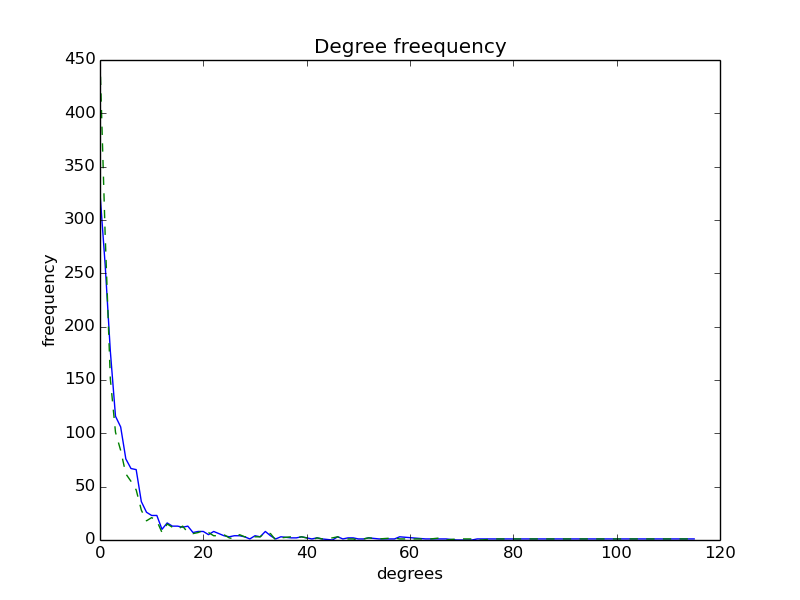
\includegraphics[width=\linewidth]{GenForestFire-1000-035-035-n1500-e7887-sketches-810-820-827-830plot}
\caption{Degree distribution graph for a natural graph using TCM sketching}
\label{fig:Degree distribution graph fora natural graph using TCM sketching}
\end{figure}

Then the automatic sketch creation is evaluated using natural graph, starting with two initial sketches of sizes 810, 820. The automatic sketch creation mechanism then created 4 more sketches with sizes 827, 830, 870, 890. Refer table \ref{tabel:Accuracy metrics for sketching with node queries on natural graphs when using automatic sketch creation}.

 
\begin{table}[!t]
\caption{Accuracy metrics for sketching with node queries on natural graphs when using automatic sketch creation}
\label{tabel:Accuracy metrics for sketching with node queries on natural graphs when using automatic sketch creation}
\centering
\begin{tabular}{|l|l|l|l|l|}
\hline
n    & e     & $G_0$=0 & $G_0$=1 & $G_0$=2 \\ \hline
1000 & 4164  & 76.0   & 82.9  & 87.4  \\ \hline
\end{tabular}
\end{table}

Finally we evaluated the large graphs with nodes 10,000 and 100,000 edges which used 4 sketches of sizes  8100, 8200, 8207, 8300. Refer table \ref{tabel:Accuracy metrics for sketching with node queries on natural graphs}.

\begin{table}[!t]
\caption{Accuracy metrics for sketching with node queries on natural graphs}
\label{tabel:Accuracy metrics for sketching with node queries on natural graphs}
\centering
\begin{tabular}{|l|l|l|l|l|}
\hline
n    & e     & $G_0$=0 & $G_0$=1 & $G_0$=2 \\ \hline
10,000 & 143,698  & 86.76   & 92.02  & 93.4  \\ \hline
\end{tabular}
\end{table}

These results shows the model is capable of working with natural graphs also, both when using automatic sketch creation and without using automatic sketch creation.

\subsection{Memory usage}
Table \ref{table:accuracy-metrics-for-sketching} shows the accuracy measures when using sketches on a 1000 nodes and 10000 edges graph. Within $\pm3$ range approximation, that is when $G_0$ is 3, there were $83.5\%$ queries giving correct results. When achieving this accuracy, the experiment used 4 sketches of sizes 810, 820, 827, 830. If we consider one cell of the adjacency matrix used one unit of memory, the the total memory used for all the 4 sketches would be, $810^2+820^2+827^2+830^2 = 2,701,329$. But if the number of nodes of the graph is knows before hand, one could create an adjacency matrix of size 1000 and that would take only $1000^2 = 1,000,000$ memory units. With sketches, the model has used approximately  2.7 times memory. 


However, as the number of nodes of the graph is not knows before hand, creating an adjacency list is not possible. If one created an adjacency matrix for N nodes, when the N+1 nodes arrives, the adjacency matrix can not accommodate the new node. But with sketching, number of nodes being larger than the sketch sizes is not a problem and the model can accommodate new nodes and still can produce an approximated result as shown in above experiments. 


One other thing is, all these sketches need not to be stored on one computation unit, but can be distributed on several units. Sketches are independent from each other, thus will not require communication between them as in graph partitioning where lot of inter partition communications happens. As the computations on sketches are independent, queries can be performed on sketches in parallel. On our sketching model, both node retrieval and edge retrieval can be done in constant time.  

\section{Conclusion}
In our study we evaluated different techniques one could use to build a graph analysis model and looking at the strengths and weaknesses of these techniques we concluded on what techniques we should continue on and  how to solve the problems of the selected techniques. We moved from graph partitioning to one pass algorithms and then to graph summarising techniques. With graph summarising techniques we considered spanner, sparsifiers and sketchers. We continued with sketchers and identified TCM as a good sketching model. Then we implemented our model using TCM sketching and evaluated  the model with different scenarios and measures. We performed node queries and edge queries with different sketching setting and evaluated the accuracy using the Average Relative Error and Number of Effective Queries as accuracy  measurement. We also evaluated if the queries we consider as Effective are really effective. Then we evaluated the confusion matrix for the queries. The results were upto a reasonable satisfactory level. 


One problem with TCM sketching was, how it suggests to create the sketches is, to use the full available  memory in order to create sketches as large as possible. We questioned can't we extend the TCM to create the sketches dynamically as the graph grows? Two problems we had to solve for this was, when to create a new sketch and how. We introduced a heuristic based technique which looks at the sketch values and decide if a new sketch should be created and a techniques to create new sketches from existing sketches. Then we evaluated them the same way. Then we discussed and evaluated how the contribution of different queries towards the accuracy of the automatic sketch creation. The system was evaluated with natural graphs and dynamic graphs for accuracy and the accuracy of the automatic sketch creation mechanism was evaluated when working with natural graphs.


In both settings, that is, with and without automatic sketch creation, edge queries could produce better results than node queries, and node queries could produce better results when the sketch sizes are closer or larger to the number of nodes of the graph. Performing edge queries and node queries in a mix, as how it happens in real world scenarios, the accuracy of the node queries  increased in automatic sketch creation setting. Thus the model best fits for system where the number of edge are relatively high than nodes and edge queries and node queries happens in a mix. As the querying on sketches can be done in parallel, the model can respond to queries faster. As we have introduces a mechanism for creating sketches on the fly, we can create new sketches only when needed.

\section{Future Works}

The automatic sketch creation mechanism should be improved with identifying better heuristics for deciding when to created a new sketch. And also should identify if any better mechanisms for creating  and  updating  new sketches exists.  

This is an embarrassingly parallel query framework model, therefore the model should be evaluated on top of a parallel framework. And also, new metrics has to be defined for thorough evaluation.




\newpage
% number - used to balance the columns on the last page
% adjust value as needed - may need to be readjusted if
% the document is modified later
%\IEEEtriggeratref{8}
% The "triggered" command can be changed if desired:
%\IEEEtriggercmd{\enlargethispage{-5in}}

% references section

% can use a bibliography generated by BibTeX as a .bbl file
% BibTeX documentation can be easily obtained at:
% http://mirror.ctan.org/biblio/bibtex/contrib/doc/
% The IEEEtran BibTeX style support page is at:
% http://www.michaelshell.org/tex/ieeetran/bibtex/
%\bibliographystyle{IEEEtran}
% argument is your BibTeX string definitions and bibliography database(s)
%\bibliography{IEEEabrv,../bib/paper}
%
% <OR> manually copy in the resultant .bbl file
% set second argument of \begin to the number of references
% (used to reserve space for the reference number labels box)
\begin{thebibliography}{1}

  \bibitem{PageRank} Page, L., Brin, S., Motwani, R.,  Winograd, T. (1998). The PageRank Citation Ranking: Bringing Order to the Web. World Wide Web Internet And Web Information Systems, 54(1999-66), 1–17. http://doi.org/10.1.1.31.1768
  \bibitem{Horawalavithana} Horawalavithana, Y. S. (2015). Cloud based publish / subscribe model for Top-k matching over continuous data streams. Undergraduate Thesis, University of Colombo
  \bibitem{TwitterStats} "Twitter: Number Of Active Users 2010-2016 | Statista". Statista. N.p., 2016. Web. 30 Dec. 2016.
  \bibitem{Facebook} Ching, A., Edunov, S., Kabiljo, M., Logothetis, D.,  Muthukrishnan, S. (2015). One Trillion Edges : Graph Processing at Facebook-Scale. Vldb, 8(12), 1804–1815. http://doi.org/10.14778/2824032.2824077
  \bibitem{WebGraphs} S. Raghavan and H. Garcia-Molina. Representing web graphs. In ICDE, pages 405–416, Atlanta, GA, USA, 2003.
  \bibitem{PowerGraph} Gonzalez, Joseph E et al. "Powergraph: Distributed graph-parallel computation on natural graphs." Presented as part of the 10th USENIX Symposium on Operating Systems Design and Implementation (OSDI 12) 2012: 17-30.

  \bibitem{Pregel}  Malewicz, Grzegorz et al. "Pregel: a system for large-scale graph processing." Proceedings of the 2010 ACM SIGMOD International Conference on Management of data 6 Jun. 2010: 135-146.

  \bibitem{Graphlab} Low, Yucheng et al. "Graphlab: A new framework for parallel machine learning." arXiv preprint arXiv:1408.2041 (2014).
  
  \bibitem{DistributedGraphLab} Low, Y., Gonzalez, J., Kyrola, A., Bickson, D.,  Guestrin, C. (2011). Distributed GraphLab: A Distributed Framework for Machine Learning in the Cloud, 716–727. http://doi.org/10.14778/2212351.2212354
  
  \bibitem{S-PowerGraph} Xie, Cong, Wu-Jun Li, and Zhihua Zhang. "S-PowerGraph: Streaming Graph Partitioning for Natural Graphs by Vertex-Cut." arXiv preprint arXiv:1511.02586 (2015).
  
  \bibitem{Graphbuilder} Jain, Nilesh, Guangdeng Liao, and Theodore L Willke. "Graphbuilder: scalable graph etl framework." First International Workshop on Graph Data Management Experiences and Systems 23 Jun. 2013: 4.
  \bibitem{Linear Embedding} Aydin, Kevin, MohammadHossein Bateni, and Vahab Mirrokni. "Distributed Balanced Partitioning via Linear Embedding." arXiv preprint arXiv:1512.02727 (2015).
  \bibitem{MinLA} Goldschmidt, Olivier, and Dorit S Hochbaum. "Polynomial algorithm for the k-cut problem." (1988): 444-451.
  \bibitem{Titan} "big graph data with cassandra - DataStax." 2012. 25 May. 2016 http://www.datastax.com/wp-content/uploads/2012/08/C2012-Titan-MatthiasBroecheler.pdf
  \bibitem{GiraphPlusPlus} Tian, Y., Balmin, A., and Corsten, S. (2013). From "think like a vertex" to "think like a graph." Proceedings of the VLDB Endowment, 7, 193–204. http://doi.org/10.14778/2732232.2732238
  \bibitem{GraphX} Xin, R. S., Gonzalez, J. E., Franklin, M. J., Stoica, I.,  AMPLab, E. (2013). GraphX: A Resilient Distributed Graph System on Spark. First International Workshop on Graph Data Management Experiences and Systems. http://doi.org/10.1145/2484425.2484427
  \bibitem{Fennel} Tsourakakis, C., Gkantsidis, C., Radunovic, B.,  Vojnovic, M. (2014). Fennel: Streaming graph partitioning for massive scale graphs. Proceedings of the 7th ACM International Conference on Web Search and Data Mining, 333–342. http://doi.org/10.1145/2556195.2556213
  \bibitem{X-stream} Roy, A., Mihailovic, I.,  Zwaenepoel, W. (2013). X-stream: edge-centric graph processing using streaming partitions. The Twenty-Fourth ACM Symposium on Operating Systems Principles, 472 – 488. http://doi.org/10.1145/2517349.2522740
  \bibitem{GraphSketches}Kook Jin Ahn, Sudipto Guha, and Andrew McGregor. 2012. Graph sketches: sparsification, spanners, and subgraphs. In Proceedings of the 31st ACM SIGMOD-SIGACT-SIGAI symposium on Principles of Database Systems (PODS '12), Markus Krötzsch (Ed.). ACM, New York, NY, USA, 5-14. DOI=http://dx.doi.org/10.1145/2213556.2213560
  \bibitem{Kalavri} Kalavri, V. (n.d.). Batch and Stream Graph Processing with Apache Flink.
  \bibitem{CountMin} Cormode, G., and Muthukrishnan, S. (2005). An improved data stream summary: The count-min sketch and its applications. Journal of Algorithms, 55(1), 58–75. http://doi.org/10.1016/j.jalgor.2003.12.001
  \bibitem{gSketch} Zhao, P., Aggarwal, C. C., Watson, I. B. M. T. J., and Ctr, R. (2011). gSketch : On Query Estimation in Graph Streams. Vldb, 5(3), 193–204. http://doi.org/10.14778/2078331.2078335
  \bibitem{TCM} Tang, N., and Chen, Q. (2016). Graph Stream Summarization From Big Bang to Big Crunch. [SIGMOD]
  \bibitem{GMatrix} Khan, A., and Aggarwal, C. (2016). Query-Friendly Compression of Graph Streams.
  \bibitem{powerLaw1}Mitzenmacher, M. (2004). A Brief History of Generative Models for Power Law and Lognormal Distributions. Internet Mathematics, 1(2), 226–251. http://doi.org/10.1080/15427951.2004.10129088
  \bibitem{powerLaw2}Xie, C., Yan, L., Li, W.-J., and Zhang, Z. (2014). Distributed Power-law Graph Computing: Theoretical and Empirical Analysis. Nips, 1673--1681. Retrieved from http://papers.nips.cc/paper/5396-distributed-power-law-graph-computing-theoretical-and-empirical-analysis.pdf
  \bibitem{frequency counts}G. S. Manku and R. Motwani. Approximate frequency counts over data streams. In VLDB, pages 346–357, 2002
  \bibitem{Vitria} Vitria. http://www.vitria.com/solutions/streaming- big-data-analytics/benefits/
  \bibitem{sparse spanners}M. Elkin. Streaming and fully dynamic centralized algorithms for constructing and maintaining sparse spanners. ACM Transactions on Algorithms,7(2):20, 2011.
  \bibitem{Spectral sparsification} J. A. Kelner and A. Levin. Spectral sparsification in the semi-streaming setting. Theory Comput. Syst., 53(2):243–262, 2013.
  \bibitem{Graph stream algorithms survey}A. McGregor. Graph stream algorithms: a survey. SIGMOD Record,43(1):9–20, 2014.
  \bibitem{HeavyHitters}G. Cormode and S. Muthukrishnan. Space efficient mining of multigraph streams. In PODS, pages 271–282, 2005.
  \bibitem{Graph sketches}Ahn, K. J., Guha, S.,  McGregor, A. (2012). Graph sketches: sparsification, spanners, and subgraphs. Proceedings of the 31st Symposium on Principles of Database Systems, 2012(Pods), 5–14.
  \bibitem{Streaming Balanced Graph Partitioning Algorithms2}Stanton, I. (2014). Streaming Balanced Graph Partitioning Algorithms for Random Graphs. Soda, 1287–1301. http://doi.org/10.1137/1.9781611973402.95
  \bibitem{Streaming Balanced Graph Partitioning Algorithms1}Kliot, G.,  Stanton, I. (2012). Streaming Graph Partitioning for Large Distributed Graphs. Acm Kdd, 1222–1230. http://doi.org/10.1145/2339530.2339722
  
\end{thebibliography}



% that's all folks
\end{document}


